\section{LINQ}

\begin{multicols*}{2}
\begin{itemize}
    \item Sprach-integrierte Abfragesprache
    \item Query-Syntax (ähnlich SQL)
    \item Beliebige Datenstrukturen als Basis (z.B. Objekte, XML)
    \item Typsicherheit
    \item Funktionale Programmierung mittels Lambda Expressions
    \item Erlaubt Deklarativen Programmierstil mittels Anonymous Types und Object Initializers
\end{itemize}
\vspace*{2mm}
\includegraphics*[width=\columnwidth]{linq}

\subsection{LINQ Extension Methods}
\begin{itemize}
    \item LINQ definiert in der Klasse Enumerable eine Vielzahl von Query Operatoren.
    \item Die Methoden in dieser Klasse stellen eine Implementierung von Operatoren zum Abfragen von Datenquellen bereit, die IEnumerable<T> implementieren.
    \item Deferred Evaluation: Query Operatoren sind ebenfalls mit yield return implementiert
    \item Immediate Evaluation: Wenn Rückgabewert nicht IEnumerable ist wird die Query sofort ausgeführt.
    \begin{itemize}
        \item ToList / ToArray
        \item Count / First
        \item Sum / Average
    \end{itemize}
\end{itemize}


\begin{lstlisting}
int[] numbers ={ 1, 4, 2, 9, 13, 8, 9, 0, -6, 12 };

IEnumerable<int> res = numbers 
    .Where(i => i >= 5) 
    .OrderBy(i => i);

IEnumerable<int> sqr = numbers
    .Skip(2)
    .Take(4)
    .Select(k=> k * k);

string[] cities = { "Bern", "Basel", "Genf", "Zürich" };

// Ausführung
List<string> citiesB = cities 
    .Where(c => c.StartsWith("B")) 
    .ToList();

// Ausführung
int citiesEndL = cities
    .Where(c => c.EndsWith("l"))
    .Count();
\end{lstlisting}

\subsection{Object / Collection Initializers}
\subsubsection{Objekte}
Mehr dazu siehe Kaptiel Klassen \& Structs $\rightarrow$ Properties $\rightarrow$ Objekt-Initialisierung.
Vor allem in Lambda Expressions häufig verwendet:
\begin{lstlisting}
int[] ids = { 2009001, 2009002, 2009003 };
IEnumerable<Student> students = ids
    .Select(n => new Student { Id = n });
\end{lstlisting}
\subsubsection{Collections}
\begin{lstlisting}
//Collections
new collection { elem1 , ..., elemN };

List<int> l1 = new() { 1, 2, 3, 4 };

//Dictionaries
new dictionary
{ 
    { key1, value1 },
    ...,
    { keyN, valueN } 
};

Dictionary<int, string> d1 = new() {
    { 1, "a" },
    { 2, "b" },
    { 3, "c" }
};

//Alternativ Dictionaries / Indexer
new dictionary
{ 
    [key1] = value1, 
    ...,
    [keyN] = valueN 
};

d1 = new() {
    [1] = "a",
    [2] = "b",
    [3] = "c"
};
\end{lstlisting}

\subsection{Anonymous Types}
\begin{itemize}
    \item Generierte Properties (Id, Name) sind readonly
    \item Anonymer Typ leitet von System.Object ab
    \item Kann nur einer Variable vom Typ var zugewiesen werden
    \item Folgende Methoden werden vom Compiler generiert
    \begin{itemize}
        \item Equals()
        \item GetHashCode()
        \item ToString() $\rightarrow$ \{ Id = 1, Name = ''John'' \}
    \end{itemize}
\end{itemize}
\begin{lstlisting}
//Syntax
new { p1 = v1, ... pN = vN };

//Verwendung
var a = new { Id = 1, Name = "John" }; 
var b = new { a.Id, a.Name };
\end{lstlisting}
Anonyme Typen für a und b sind identisch (Wiederverwendung)

\subsection{Query Expressions Einführung}
SQL-ähnliche Syntax
\begin{lstlisting}
// 1. Datenquelle wählen
int[] numbers = { 0, 1, 2, 3, 4, 5, 6 };

// 2. Query erstellen
var numQuery =
    from num in numbers
    where (num % 2) == 0
    select num;

    // 3. Query ausführen
foreach (int num in numQuery) {
    Console.Write("{0,1} ", num);
}    
\end{lstlisting}
\subsubsection{Übersetzung in Lambda Expressions}
Query Expressions werden vom Compiler in Lamda Expressions umgewandelt.
\begin{lstlisting}
var q1 = from s in Students
    where s.Subject == "Computing"
    orderby s.Name
    select new { s.Id, s.Name };
\end{lstlisting}
\subsubsection{Syntax}
\begin{itemize}
    \item from: Definiert eine Range-Variable und eine Datenquelle
    \item where: Filter
    \item orderby: Sortierung
    \item select: Projektion auf einen Elementtypen
    \item group: Gruppierung in eine Sequenz von Guppen-Elementen
    \item join: Verknüpfung zweier Datenquellen
    \item let: Definition von Hilfsvariablen
\end{itemize}
\fat{Regeln:} Beginnt immer mit ''from'' endet immer mit ''select'' oder ''group''

\subsection{Query Expressions Abfragen}
\includegraphics*[width=\columnwidth]{linq2}
\subsubsection{Range Variabeln}
\begin{itemize}
    \item Enstehen durch folgende Klauseln: from / join / into
    \item Sind readonly
    \item Müssen unterschiedlich der äusseren lokalen Variablen benannt werden
    \item Innerhalb der Expression und bis zur nächsten ''into'' Klausel sichtbar
\end{itemize}
\begin{lstlisting}
from s in Students
join m in Markings on s.Id equals m.StudentId 
group s by s.Subject into g
select g;

//Students: IEnumerable<Student>
//s: Student
//Markings: IEnumerable<Markings> 
//m: Markings
\end{lstlisting}
\subsubsection{Gruppierung}
\begin{itemize}
    \item Transformation in Key/Value Pairs
    \item Zusammenfassung in ein IEnumerable der Gruppen nach Key
    \item Gruppierung in IGrouping<TKey,TElement>
\end{itemize}
\begin{lstlisting}
//q: IEnumerable<IGrouping<string, string>>
var q = from s in Students
    group s.Name by s.Subject;  

foreach (var group in q)
{
    Console.WriteLine(group.Key);
    foreach (var name in group)
    {
        Console.WriteLine("  " + name);
    }
}

//Ausgabe Beispiel
Computing
    John
    Adam
Mathematics
    Sarah
    Peter
\end{lstlisting}
\fat{into:}
\begin{itemize}
    \item ''into'' speichert Resultat in Variable g
    \item ''s'' ist danach nicht mehr sichtbar
    \item ''g'' kann als Gruppe weiterverwendet werden
\end{itemize}
\begin{lstlisting}
var q = from s in Students
group s.Name by s.Subject into g
select new
{ 
    Field = g.Key,
    N = g.Count()
};

foreach (var x in q)
{
    Console.WriteLine(x.Field + ": " + x.N); 
}

//Ausgabe
Computing: 2 
Mathematics: 2
\end{lstlisting}
\subsubsection{Inner Joins / Method Syntax}
\begin{lstlisting}
var parents = new List<Parents> { new(), new() };
var children = new List<Child> { new(), new() };

var parentsWithBirtdateOfChild = parents //table1
    .Join(
        children, //table2
        p => p.Pid, //primary key
        c => c.Pid, //foreign key
        (parent, child) => new //result
        {
            KundenName = parent.Name,
            BestellDatum = child.Birthdate
        }
    );
\end{lstlisting}
\subsubsection{Inner Joins / Explizit}
\begin{itemize}
    \item Verknüpft zwei Mengen über einen Schlüssel
    \item Zwingend mit ''equals'' verknüpfen (nicht mit ==)
\end{itemize}
\begin{lstlisting}
var q =
    from s in Students
    join m in Markings
    on s.Id equals m.StudentId
    select s.Name + ", " + m.Course + ", " + m.Mark;

//Ausgabe
John Doe, Programming, 3
John Doe, Databases, 2
John Doe, Computer Graphics, 1 
Linda Miller, Organic Chemistry, 1
\end{lstlisting}
\subsubsection{Inner Joins / Implizit}
\begin{itemize}
    \item Verknüpft zwei Mengen über einen Schlüssel
    \item Unterschied: Weniger effizient
    \item Bildetr Kreuzprodukt
\end{itemize}
\begin{lstlisting}
var q =
    from s in Students
    join m in Markings
    on s.Id == m.StudentId
    select s.Name + ", " + m.Course + ", " + m.Mark;

//Ausgabe
John Doe, Programming, 3
John Doe, Databases, 2
John Doe, Computer Graphics, 1 
Linda Miller, Organic Chemistry, 1
\end{lstlisting}
\subsubsection{Group Joins}
\begin{itemize}
    \item Pro Student wird eine Liste für alle Markings erstellt
    \item s bleibt sichtbar
\end{itemize}
\begin{lstlisting}
var q =
    from s in Students 
    join m in Markings
        on s.Id equals m.StudentId
    into list
    select new
    {
        Name = s.Name,
        Marks = list
    };

foreach (var group in q) 
{
    Console.WriteLine(group.Name);
    foreach (var m in group.Marks)
    {
        Console.WriteLine(m.Course);
    }
}
\end{lstlisting}
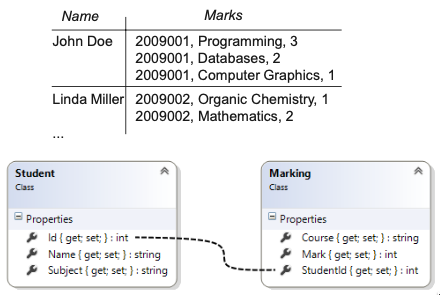
\includegraphics[width=.75\columnwidth]{linqexmp}
\subsubsection{Left Outer Joins}
\begin{itemize}
    \item Verknüpft zwei Mengen über einen Schlüssel
    \item Wenn kein rechtes Element gefunden wird bleibt linkes Element trotzdem bestehen
\end{itemize}
\begin{lstlisting}
var q =
    from s in Students 
    join m in Markings
        on s.Id equals m.StudentId
    into list
    from sm in list.DefaultIfEmpty()
    select s.Name + ", " + (sm == null
        ? "?"
        : sm.Course + ", " + sm.Mark);

foreach (var x in q)
{ Console.WriteLine(x); }

//Ausgabe 
John Doe, Programming, 3
John Doe, Databases, 2
John Doe, Computer Graphics, 1 
Linda Miller, Organic Chemistry, 1 
Ann Forster, ?
\end{lstlisting}
\subsubsection{let}
\begin{itemize}
    \item Erlaubt das Definieren von Hilfsvariablen
\end{itemize}
\begin{lstlisting}
var result =
    from s in Students
    let year = s.Id / 1000
    where year == 2009
    select s.Name + " " + year.ToString();

foreach (string s in result)
{
    Console.WriteLine(s);
}

//Ausgabe
John Doe 2009 
Linda Miller 2009 
Ann Foster 2009 
Sam Doug 2009
\end{lstlisting}
\subsubsection{Select Many}
\begin{itemize}
    \item Erleichtert das Zusammenfassen verschachtelter Listen
    \item Führt für jedes Listenelement auf oberster Stufe den selector aus
    \item Dieser liefert selbst eine Liste (Teilliste)
    \item Teillisten werden untereinander gehängt
\end{itemize}
\begin{lstlisting}
List<List<string>> list = new() {
    new() { "a", "b", "c" },
    new() { "1", "2", "3" },
    new() { "ö", "ä", "ü" }
};

var q1 = list.SelectMany(s => s);
//Gleichbedeutend wie
var q2 =
    from segment in list
    from token in segment
    select token;

foreach (string line in q1)
{ Console.Write("{0}.", line); }

//Ausgabe
a.b.c.1.2.3.ö.ä.ü.
\end{lstlisting}
\end{multicols*}